\documentclass{sig-alternate}
\usepackage{url}

\title{FriendlyLocation: Using Tie Strength to Geo-locate Users
}
\numberofauthors{1} 
\author{
    \alignauthor Jeffrey McGee, James Caverlee\\
    \affaddr{Department of Computer Science and Engineering, Texas A\&M
    University} \\
    \affaddr{ College Station, TX 77845 USA} \\
    \email{jeffamcgee@tamu.edu, caverlee@cse.tamu.edu}
} 
\begin{document}

\maketitle
\begin{abstract}
With the rise of volunteered user location information through services like
Foursquare, Google Latitude, and Facebook Places, we face unprecedented access
to the trails and connections among millions of social media users. This
location information is increasingly being incorporated in social media for
providing localized content, location-aware recommendations, and other
geo-spatial enabled services. In this paper, we investigate the interplay of
distance and tie strength through an examination of 20 million geo-encoded
tweets collected from Twitter and 6 million user profiles. Concretely, we
investigate the relationship between the strength of the tie between a pair of
users, and the distance between the pair. We identify several factors --
including following, mentioning, and actively engaging in conversations with
another user -- that can strongly reveal the distance between a pair of users.
We find a bimodal distribution in Twitter, with one peak around 10 miles from
people who live nearby, and another peak around 2500 miles, further validating
Twitter's use as both a social network (with geographically nearby friends) and
as a news distribution network (with very distant relationships). Based on
these findings, we propose and evaluate a method for predicting location for
users based purely on an analysis of the user's social network, which has great
significance for augmenting traditional social media and enriching
location-based services with more refined and accurate location estimates.

\end{abstract}




\section{INTRODUCTION}



Publicly available data.
@mention
efficient


\section{RELATED WORK}
\cite{scellato2011socio}
\cite{scellato2010distance}
\cite{backstrom2010find}
\cite{cheng2010you}
Gilbert ?


\section{DATA COLLECTION}
We collecetd 

social networking and blogging sites.

We define the set of the user's friends, followers, and the users who they mention to be their contacts.
Twitter does not provide a mechanism to deteremine who mentioned a given user, and as a result, we do not consider these users to be contacts.
In some blogging platforms, such as Tumblr, it is relatively easy to find the communication edges that point back toward a user.
In those platforms, it would be fairly straightforward to use that information in location prediction.

Any given contact can be categorized into precisely one of these four disjoint sets:
\begin{description}
\item[reciprocal friend (rfrd)] The geo-located user follows this user and is followed back.
\item[just friend (jfrd)] The geo-located user follows this user and is not followed back.
\item[just follower (jfol)]The geo-located user is followed by this user, but does not follow them.
\item[just mentioned (jat)] The users do not follow each other, but the geo-located user mentioned the name of the other user in a tweet.
\end{description}

We used Twitter's Streaming API to obtain 19877804 tweets that contain
geographic information and were posted between April 7 until April 16,2011.
We ignored tweets from users who made their account private, had neither
friends nor followers, or posted fewer than two tweets in the sample.
We found the median latitude and median longitude for each user, and use this
as an approximation of the home location of the user.
We noticed that some Twitter accounts, such as accounts that posted jobs, would
move around faster than a human could possibly move. To account for this, we
calculated the distance between each tweet and the user's home location. We
ignored users if the median distance from their tweets to their home location
was greater than 50 miles.

We considered users to be in the US based on a simple bounding box.  If their median latitude was between 24 and 50 degrees and their median longitude was between -126 and -66 degrees, then their home location was considered inside the continental US.
We divided these geo-located users into groups based on the last digit of their twitter user id:
\begin{description}
\item[0--6] The training group had 104214 users with a home location in the US bounding box. Some of these users were also used to evaluate the quality of geocoding. For geocoding, we chose users from around the world with a decodable location field and split them into two groups:
\begin{description}
\item[0--3] The geocoding training group has 131295 users.
\item[4--6] The geocoding evaluation group has 85664 users.
\end{description}
\item[7--9] The evaluation group had 40861 users with a home location in the US.
\end{description}

For all of the geo-located users who lived in the US, we used Twitter's API to download the users' friends, followers, and 100 most recent tweets.
We also downloaded the profiles for up to 2000 friends, followers, and people they mention in their tweets. If they had over 2000, we chose a random sample of 2000 profiles that included at least 25 of each of the four categories listed below.
From the profiles, we kept the users with a decodable location field and threw away the rest. From what was left, we randomly picked one contact from each of these four categories of contacts defined in the Introduction.
For each of these contacts, we stored their friends, followers, and 100 most recent tweets.

\subsection{Geocoding}
We used Gisgraphy\footnote{\url{http://www.gisgraphy.com/}} to do geocoding.
Gisgraphy does full-text search on the GeoNames\footnote{\url{http://www.geonames.org/}}
database using Lucene. Since
it runs locally we are not limited to a certain number of queries per day.
Gisgraphy's geocoder returns ranked results based on a full text search
over millions of geographical features such as countries, cities, and schools. 

The location field on a user's profile is just a text field that asks the user to respond to "Where in the world are you?".
Responses vary from precise latitude and longitude coordinates entered automatically by smart phone apps to jokes and nonsense.
We had to do some preproccessing before sending user-submitted locations to the geocoder.
First, we used a regular expression to find latitude and longitude coordinates. These are treated as if they were a unique type of location returned by the geocoder.
Occasionally, users would put two locations separated by a slash, dash or a conjunction. If the geocoder did not return any results for a user, we tried to geocode both locations and used the first location that the geocoder understood.

We noticed that some locations are significantly more useful than others.
For example, even though Rhode Island and Montana are both states with around
one million people, Rhode Island is smaller, and as a result, much more useful
in estimating the location of a user.
To make the results of the geocoder more useful, we devised a method to estimate the accuracy of a location returned by the geocoder.
For the users in the geocoding training and evaluation groups, we have both the
home location based on geo-located tweets, and the free-response location field
that we did geocoding on.
Originally, we planned to just use the users in the US, but we found that users
in the US had friends outside of the US, so we need to estimate the quality of
locations outside of the US as well.
As a result, we trained on geographic data from around the world.

We define the location error to be the distance between a user's home location and the result from the geocoder.
The location error can vary from less than a mile to over ten thousand miles.
We ran the geocoder on each user in the geocoding training group, and then grouped users based on the result of the geocoder.
For the 3866 locations that had at least three users, we calculated the median location error for that location.
Next, we grouped all of the locations that had the same type and had one or two users, and calculated the median error for the location type.
We choose the median over average or standard deviation because those metrics are strongly affected by large outliers.
We choose to make the cutoff three because that is the smallest value where the median is not just an average.
Table \ref{tab:MedianLocErr} shows the median location error for a few example locations and location types.

We now have a method to predict the quality of a coordinate returned by Gisgraphy.
We define the predicted location error(PLE) for a given location to be median location error if it is one of the 3866 locations that had three users; otherwise, it is the median location error for the location's type.
For example one user had "PDX,OR" in his location field. Gisgraphy identifies this as "Portland International Airport". Since it is not one of the most common locations, its PLE is determined by its place type to be 31 miles as seen in Table \ref{tab:MedianLocErr}.

In Figure \ref{fig:DiffGnpGps}, we show the result of using the PLE to ignore users who have low quality locations such as "Pluto".
The solid black line represents the normal results of geocoding where the location error is less than 1000 miles for 88\% of the users.
The cyan line represents what happens when we remove locations with a PLE greater than or equal to 1000 miles. Now, after removing only 6\% of the users, 93\% of them are within 1000 miles.

\begin{table}
\centering
\caption{Example Median Location Errors}
\begin{tabular}{l r r} 
Location&Number of Users&Median Error in Miles\\ \hline
``Bronx''&53&4\\
``New York''&1264&174\\
``Pluto''\footnote{According to Gisgraphy, Pluto is a city in the Philippines and not a planet.}&11&7843\\ \hline
\\
Place Type&Number of Users&Median Error in Miles\\ \hline
A Coordinate&25216&3\\
A City&7128&6\\
An Airport&117&31\\
A Country&37&3935\\
\hline\end{tabular}
\label{tab:MedianLocErr}
\end{table}

\begin{figure}
\centering
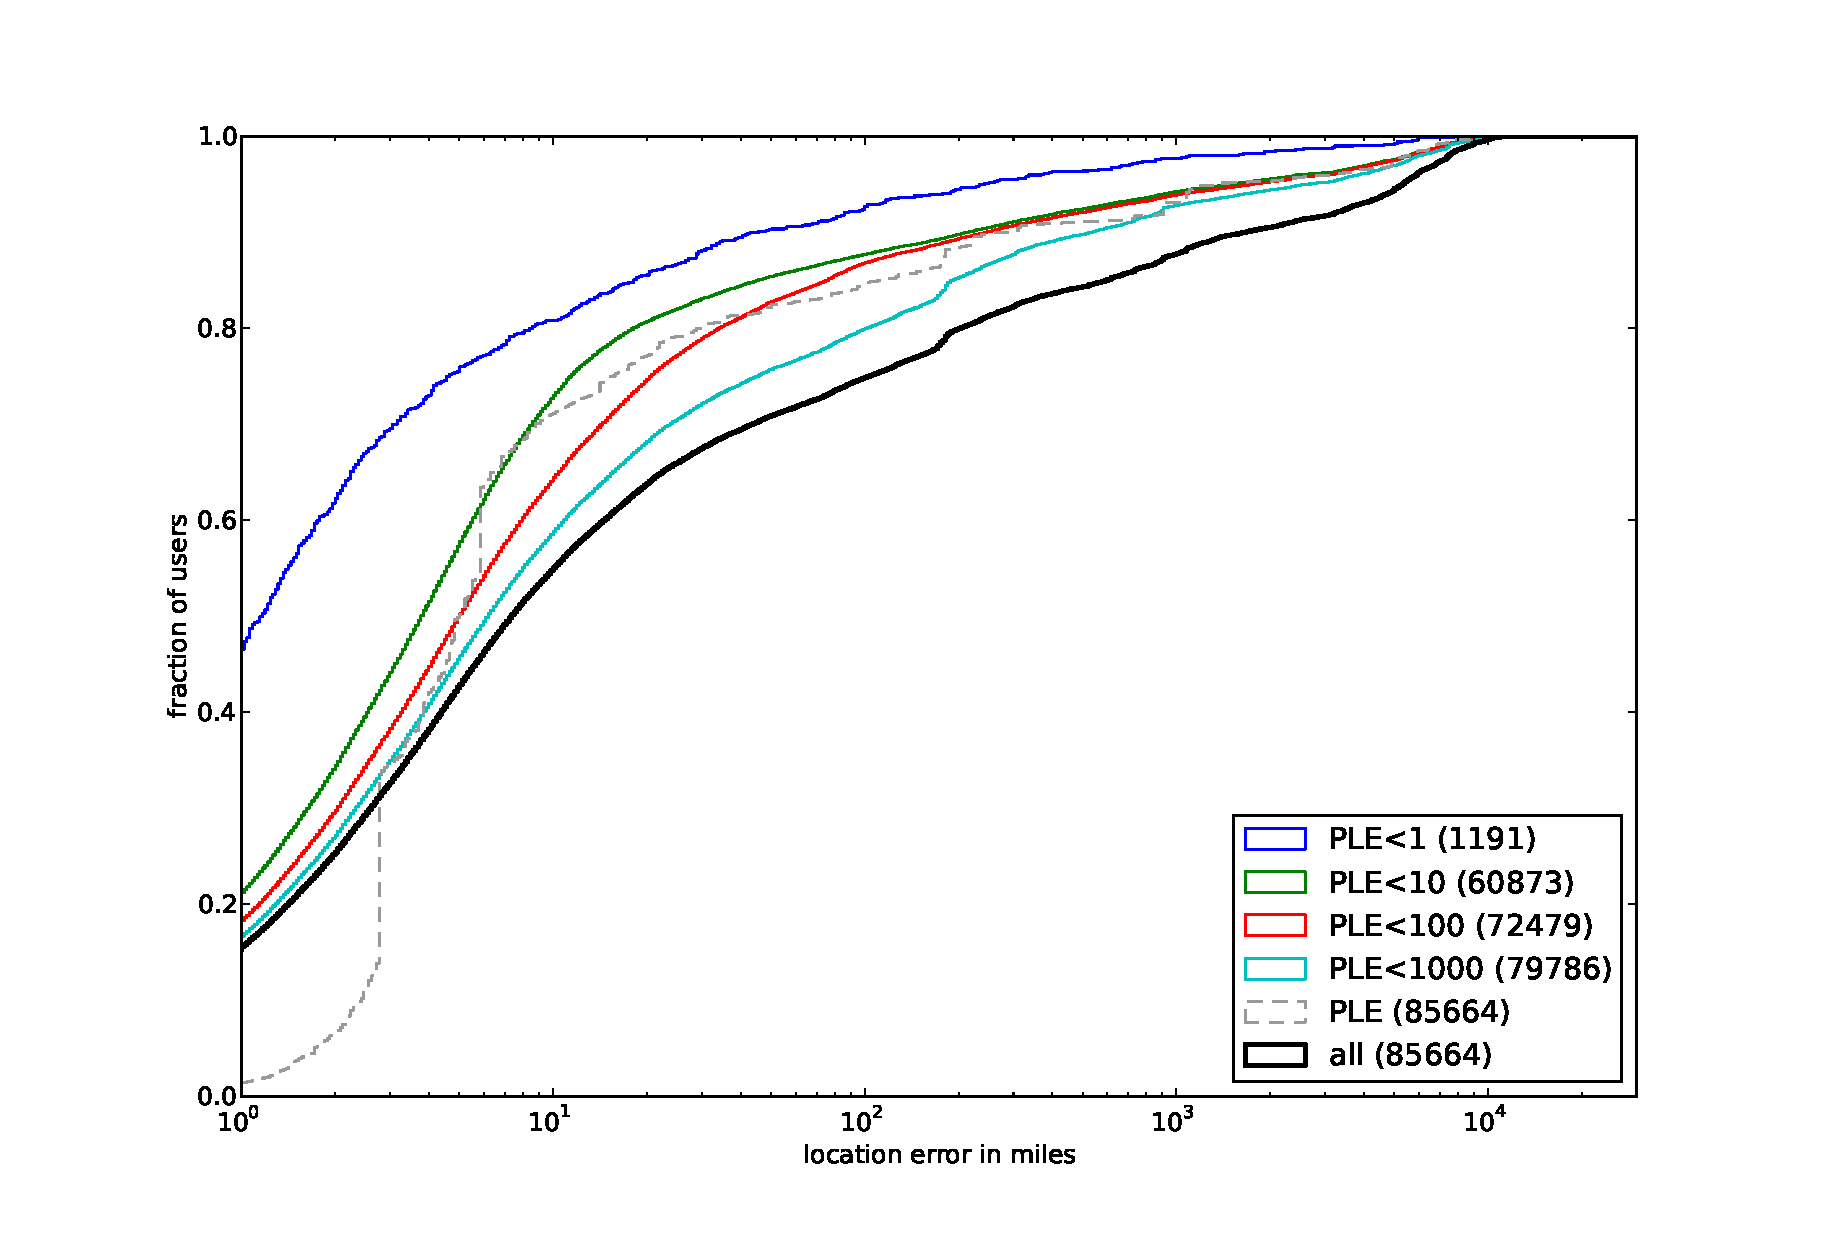
\epsfig{file=diff_gnp_gps.eps, width=\linewidth}
\caption{
The dashed line shows the cumulative distribution function(CDF) of the predicted location error.
The other lines show the CDF of the actual location error for the geocoding evaluation group. The colored lines show how the location prediction improves when we remove users with a high PLE. For example, all the users in the "PLE<1" category have a predicted location error(PLE) of less than one mile.
In the legend, the number in parenthesis is the number of users in that category.
}
\label{fig:DiffGnpGps}
\end{figure}


\begin{figure*}
\centering
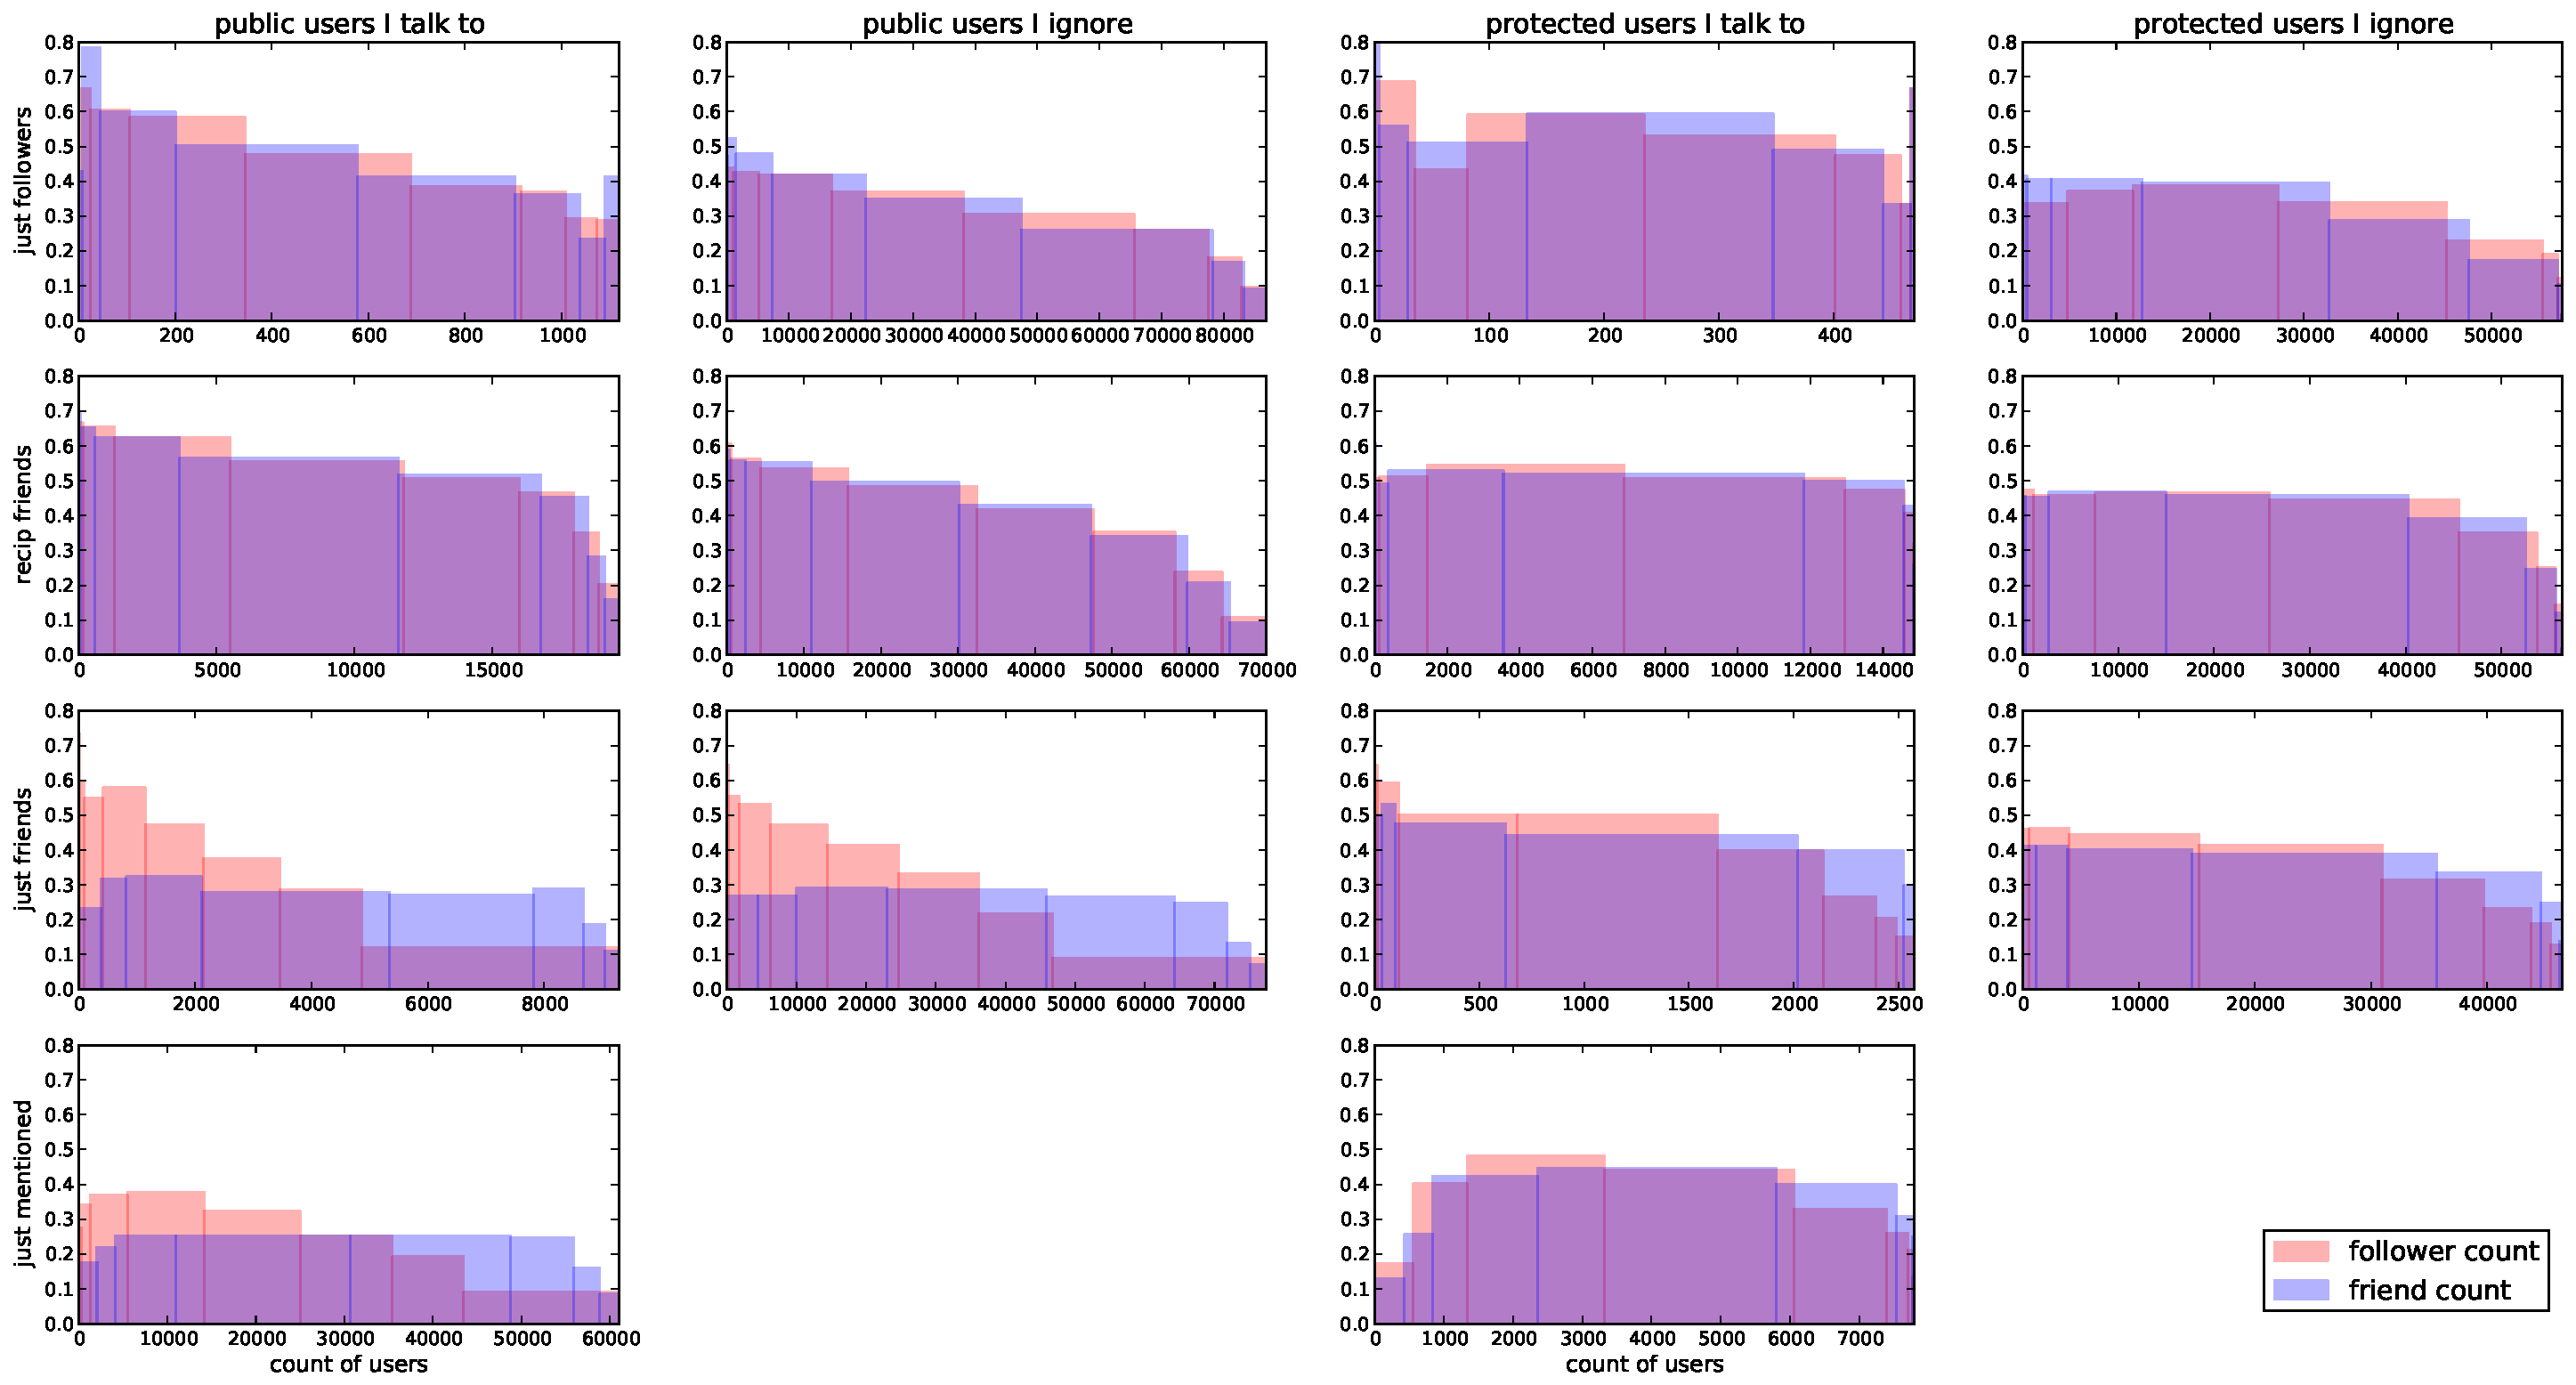
\epsfig{file=local_all.pdf, width=\linewidth}
\caption{
Hi!
}
\label{fig:LocalAll}
\end{figure*}

\section{INVESTIGATION}
Every user who has multiple contacts will have some people who are much
closer than others. In order to estimate the locations of users, we would like
to find out which users are most likely to live nearby.  In this section, we
investigate how various types of contacts correlate with proximity.
All of the analysis in this section was done on the 104214 users with a home location inside the US bounding box. We used their friends, followers, and the people they mention with a PLE of less than 1000 miles.

\subsection{What type of contact is closest?}
\begin{figure}
\centering
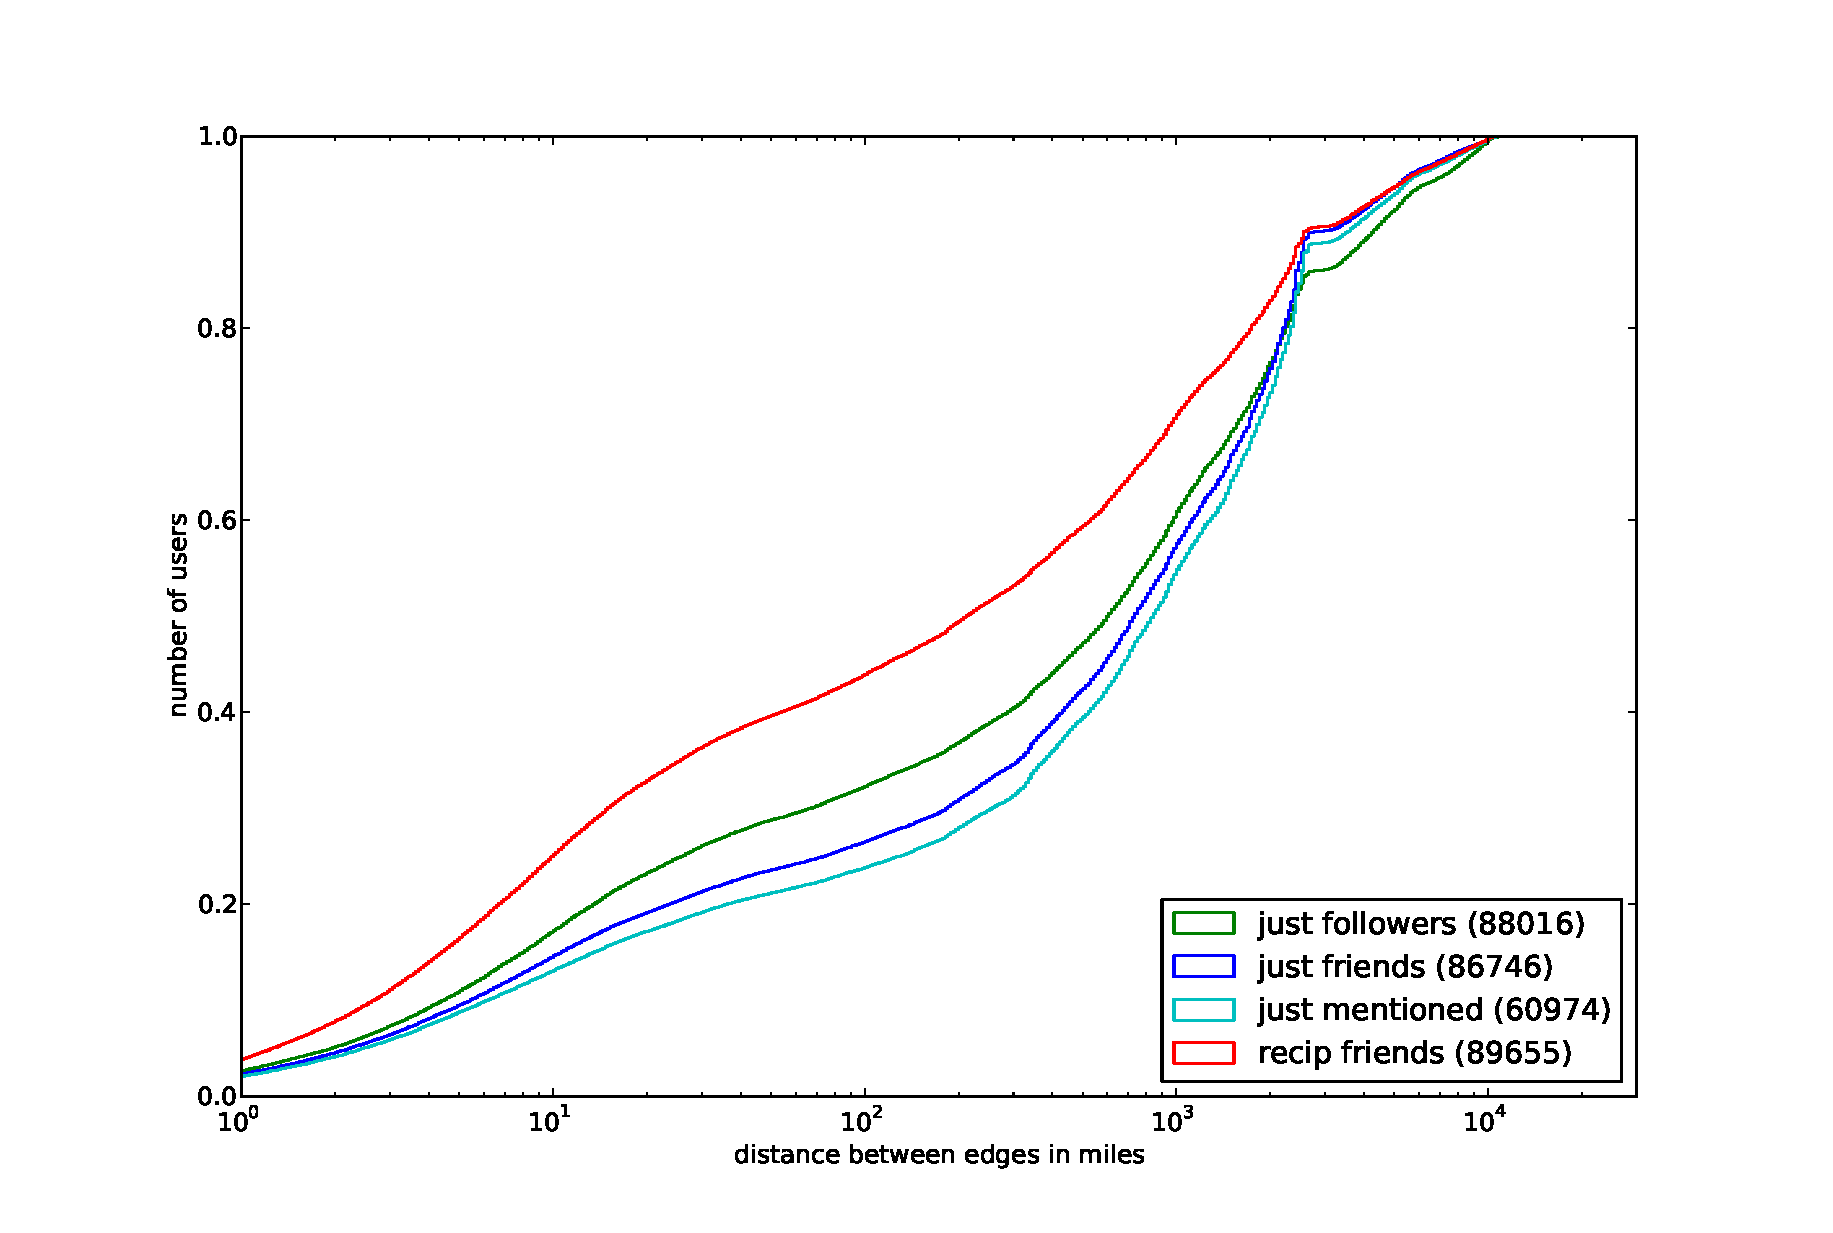
\epsfig{file=edge_types_cuml.eps, width=\linewidth}
\caption{
CDF of distance from geo-located users to users they have some contact
with.
}
\label{fig:EdgeTypesCum}
\end{figure}
In Figure \ref{fig:EdgeTypesCum} we look at the cumulative distribution function(CDF) of the distance between a geo-located user and several types of contacts.
Reciprocal friends are the closest, followed by followers, friends, and finally users who are just mentioned.
While it may seem that since being followed by someone and following someone should be identical, they are not.
Famous users on Twitter often have large numbers of followers, but they do not follow a large number of users back.
Since the geo-located user was selected randomly, they are usually an average user and not a celebrity.
If they follow someone, it might be a celebrity; however, if someone follows them, it is probably someone who knows them.

There is a strange corner in the top right corner of all the graphs at approximately 2500 miles. This is caused by the large population living on the coast, and the tiny number of people posting tweets from the Atlantic and pacific oceans.

\subsection{What is the distribution of related users?}
\begin{figure}
\centering
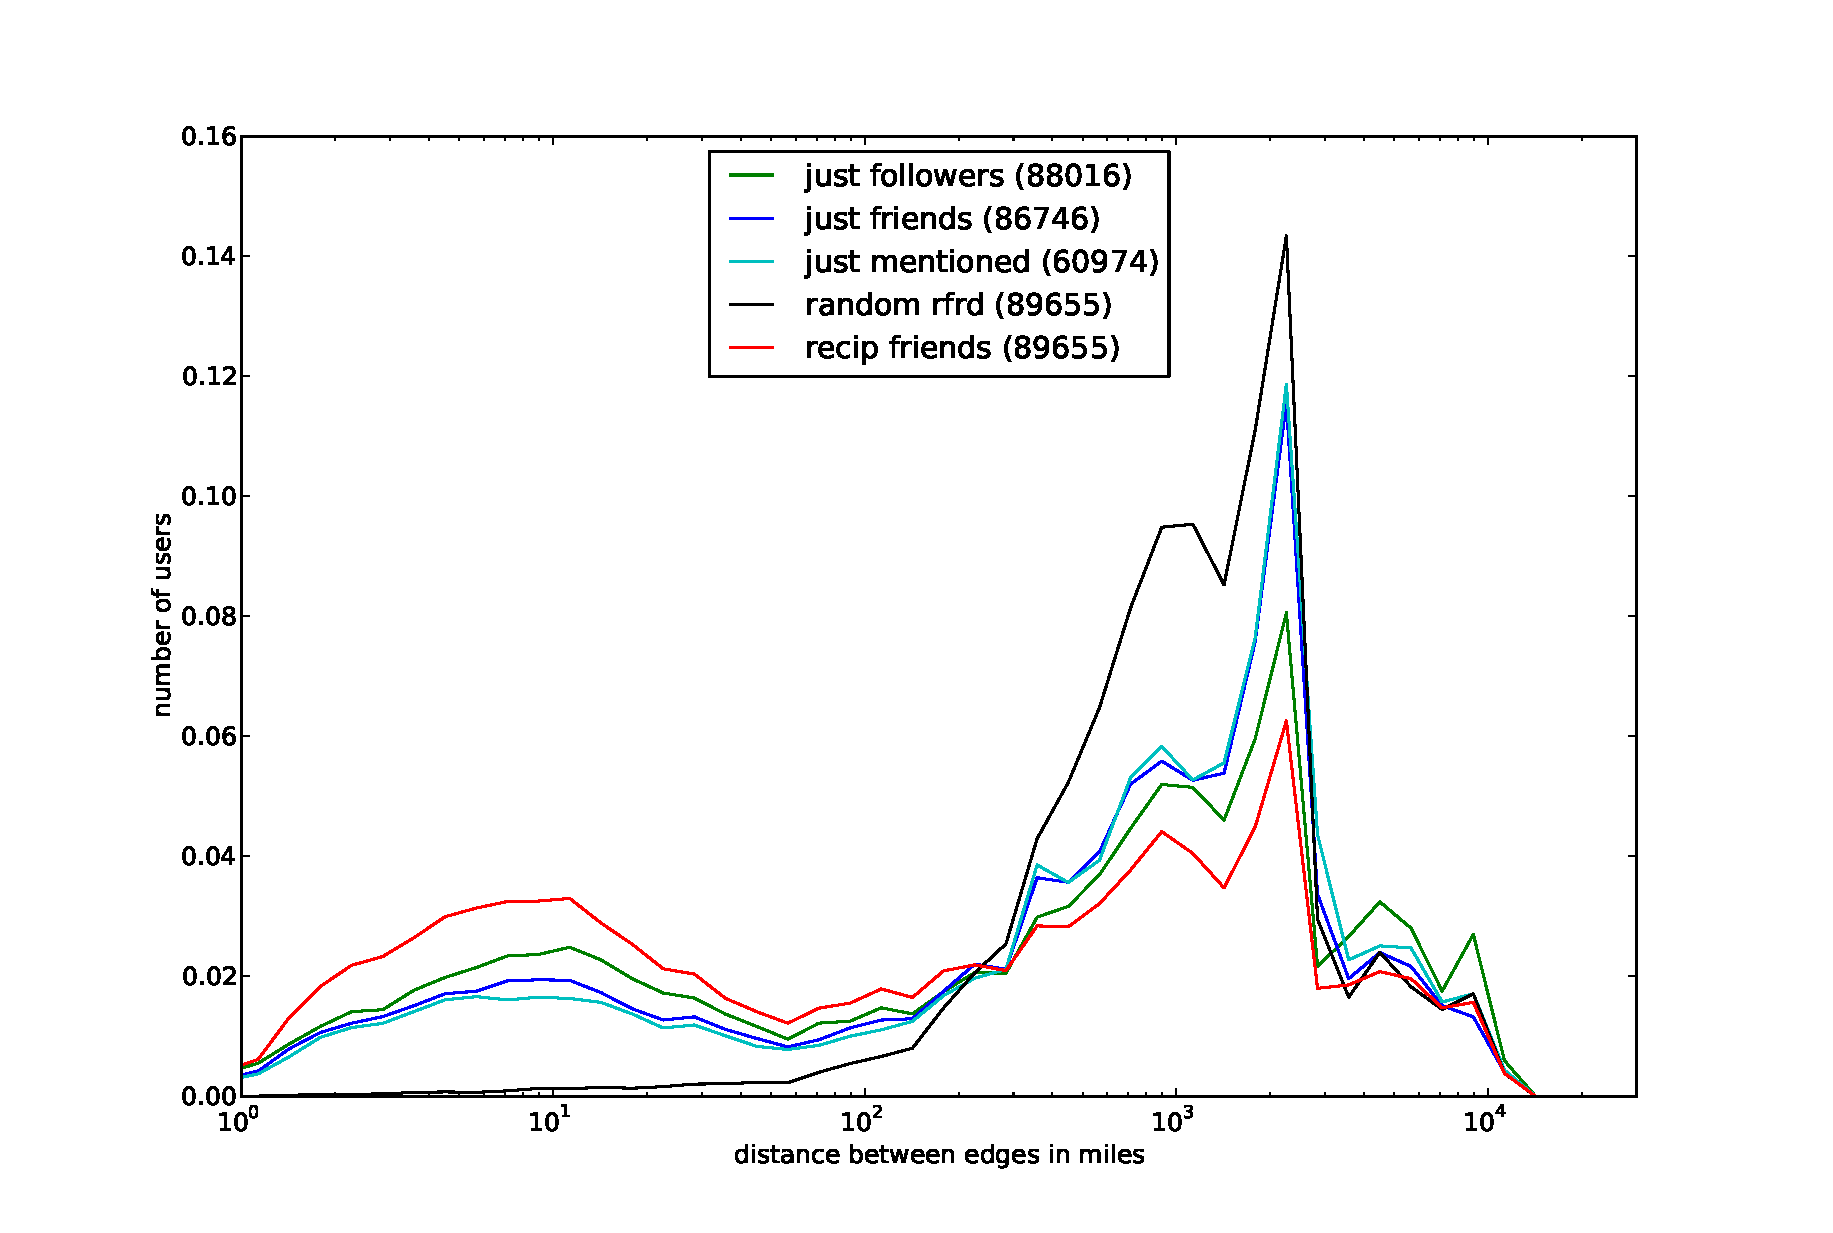
\epsfig{file=edge_types.eps, width=\linewidth}
\caption{
Smoothed histogram of distance to users.  The curves in Figure
\ref{fig:EdgeTypesCum} are the integrals of these curves. The black line was created by calculating the distance between random, unrelated users. Notice how it has a similar shape to the other curves for distances greater than 100 miles.
}
\label{fig:EdgeTypes}
\end{figure}
Instead of looking at the CDF, we will now turn our attention to Figure
\ref{fig:EdgeTypes}: a smoothed histogram of the distance to related users.
Distance is once again plotted on a logarithmic scale to show both local and
global effects.
All four types of contacts follow roughly the same bimodal distribution:
one peak around 10 miles from people who live nearby, and another peak around
2500 miles.
\textsc{reference chart in bracstrom paper here}

The red line in Figure \ref{fig:EdgeTypes} is based on the distance between
89655 geo-located users and their reciprocal friends. We shuffled the
geo-located users so that they would be paired with someone who was probably
not their friend and then calculated the distance between them. The black line
shows the results of this procedure. For distances greater than around five
hundred miles, the red line and the black line have roughly the same shape,
which suggests that people when people are far away, their physical location no longer matters.

One reasonable explanation for this is that Twitter is not just a social
network; it is also an news distribution network.  This bimodal distribution
suggests that users have two types of contacts: people who they met in
real life, and people who they met online or know about via mainstream media.
The former group is useful for predicting location and the latter group is not.

\subsection{What is the effect of communicating with someone?}

\subsection{Are you closer to private accounts?}
\begin{figure}
\centering
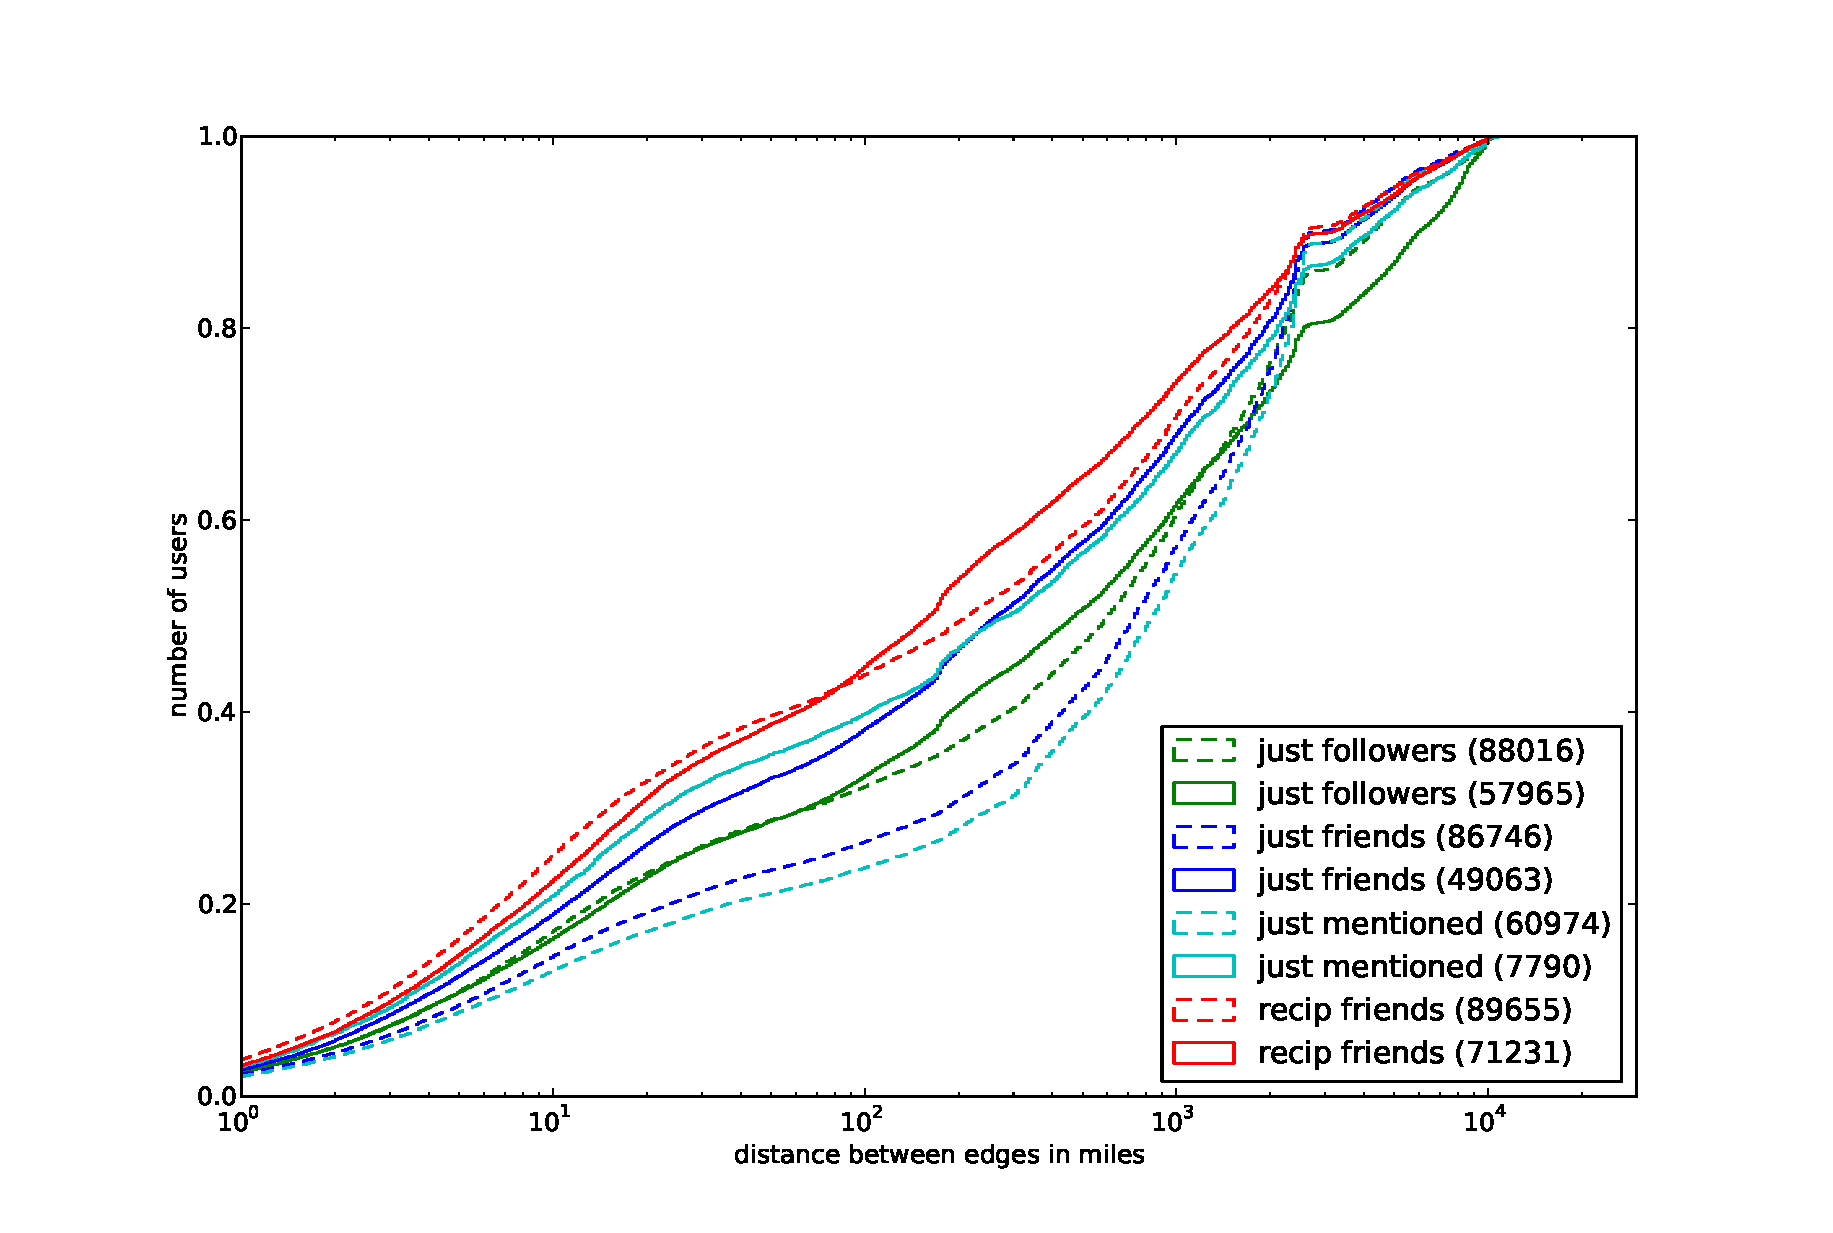
\epsfig{file=edge_types_prot.eps, width=\linewidth}
\caption{ Solid lines represent protected accounts, and dashed lines represent
public accounts. If a user follows a protected account, they tend to be closer.}
\label{fig:EdgeTypesProt}
\end{figure}

Like many social networks, Twitter allows users to mark their account as protected. The specifics differ from network to network, but in Twitter's case a user has to be approved to follow a protected user.
In most of this section we are only concerned with public accounts, but in this subsection, we investigate how protected accounts compare to public accounts.

The most dramatic difference between private and public occurs if a user follows a protected account.
Since users generally only allow people they know to follow a protected account, this brings the users almost as close together as if they were reciprocal friends. On the other hand, if a protected account follows the geo-located user, this is almost insignificant.

One possible explanation for the \textsc{red lines crisscrossing} is that a protected account is more likely to live in a rural, unpopulated area. \textsc{cite Gilbert}

\subsection{If two mutual friends live near each other, does that increase the chance that they live near you?}
yes, but it doesn't matter

\subsection{Does the type of triangle matter?}

The number of triangles formed is NOT a function of the number of edges a user has; therefore talking about the ratio of people involved in a type of triangle is stupid.

star
mutual fan
path
loop 
star v. non-star matters a lot for friend case, but not so much in others



\subsection{Are you closer to people you communicate with?}
yes

\subsection{Does the number of friends and followers a person have affect how close they are?}


\section{RELATIONSHIP MODEL}
\label{sec:model}

Power law


\section{EVALUATION}
\subsection{Procedure}
The geolocated users we used to do the evalutation are less concerned about the
privacy of their location information than the average twitter user.
As a result, they tended to give better information in the location field of
their user profile than the average twitter user.
For this evaluation we choose to ignore the contents of the geolocated user's
location fields.

We evaluated the FriendlyLocation system against 40831 of the 40861 users from the evaluation group.
We removed thirty users from this set because none of their friends or
followers had decodable locations.
(When we initially created the evaluation
set we removed users with both zero friends and zero followers.)

We investigate several implementations of the FriendlyLocation sytem:
\begin{description}
\item[Full] This is the system described in the previous section.
\item[Location Error] This shows the value of calculating the median location error.
\item[Relationship Types] Returns the contact that is physically closest to the user.
\item[Simple] This system treats all contacts equally---we ignore their median location error and 
\end{description}

In adddition to using the FriendlyLocation system as described in the previous section, we created a few baseline location predictors:
\begin{description}
\item[Median] Finds the median of the latitude and the median of the longitude of the user's contacts.
\item[Mode] Finds the most common location of the user's contacts, and breaks ties by picking one randomly.
\item[Omniscient] Finds the contact that is closest to the user.
\end{description}

\subsection{Results}

It works! Kinda.

\section{FUTURE WORK}
combine other factors

\bibliographystyle{abbrv}
\bibliography{fl} 
\end{document}
